\documentclass{sig-alt-release2}
\usepackage{graphicx}
\usepackage{url}
\usepackage{textcomp}
\usepackage{times}
\usepackage{color}

\newcommand{\todo}[1]{}
% \newcommand{\todo}[1]{\footnote{{\bf TODO:} #1}}
\newcommand{\Intel}{Intel\textsuperscript{\textregistered}}

\newcommand{\idea}[1]{{\color{blue} IDEA: #1}\\}
\newcommand{\studyresult}[1]{{\color{red} STUDY RESULT?: #1}\\}

\begin{document}
%
\title{Connecting Documents to Ideas}

\numberofauthors{3}

\author{
\alignauthor Beth Trushkowsky\\
       \affaddr{Computer Science Division}\\
       \affaddr{University of California at Berkeley}\\
       \email{trush@berkeley.edu}
\alignauthor Rob Ennals\\
       \affaddr{Intel Research}\\
       \affaddr{2150 Shattuck Avenue}\\
       \affaddr{Penthouse Suite}\\
       \affaddr{Berkeley, CA 94704, USA}\\
       \email{robert.ennals@intel.com}
}

\sloppy 

\maketitle

\begin{abstract}

Much of the information contained on the web consists of opinions, arguments, blogs, articles, and other such unstructured natural language text. Each such document contains one or more statements or ideas that might be of interest to readers.

We propose a new approach to finding, organizing, and sharing ideas contained in web pages. In this approach, a user marks points of interest 

\end{abstract}

\section{Introduction}
1p:  
overview, 
motivation,
list of contributions,
(briefly) describe application,
(briefly) describe user studies,
describe results,

% \idea{Much interesting data on the web is unstructured text}
% 
% \idea{These documents consist of ideas}
% 
% \idea{Think Link connects documents to the ideas they express}
% 
% %\idea{This paper is itself marked up in think link - with URL}
% 
% \idea{If the ideas in a document are known then this allows interesting queries}

% Motivation for tool

% What thinklink allows people to do

% Why thinklink is needed
\section{Motivation?}
1-2pp: 
how do people currently organize, interact, share with web content; 
Thinklink data structures; 
what can people now do with Thinklink

\subsection{Why People Annotate}

\idea{People already annotate documents, in the form of blogs, comments etc}

\idea{People already organize data, using text files, Google Notepad, OneNote, etc}

\idea{People already share information, by mailing links, posting stories on facebook, sending messages on twitter, etc}

\idea{People already want to see what each other are interested in - using Facebook, Twitter, Friendfeed, etc}

\studyresult{Our users used these tools}

\studyresult{Users want to put forward their opinions}

\studyresult{People want to be seen as a source of useful information}

\studyresult{People want to organize the information they find}

\studyresult{Our users said they would use our tool}

%\studyresult{The best way to find answers is social - by learning from friends who understand the topic}


\subsection{Organizing Knowledge}

\idea{Like Wikipedia without the articles}

\idea{Organize ideas with Points, snippets, and topics}

\idea{A point can support or oppose another point}

\idea{A point can be exactly the same or exactly opposite}

\idea{Important to have wiki features to keep things in check}

\studyresult{People found it useful to organize ideas}

%\studyresult{People found the topic approach worked well}

%\studyresult{People were able to easily find and reuse existing points and topics}


\subsection{Using this Knowledge}

\idea{Show me the points that other people disagree with}

\idea{Show me the points that other people found interesting}

\idea{Show me the points that my friends found interesting}

% future queries want to support

\idea{Show me the articles that make interesting points I haven't heard before}

\idea{Show me when new snippets appear on points I'm interested in}

\idea{Show me when new points appear on topics I'm interested in}


%\studyresult{People liked to be able to monitor interesting new ideas on topics they were interested in}

\studyresult{People liked the other features too}

\section{Design}
2pp: describe how the application works and show some screenshots; discuss some implementation decisions
\subsection{Features}
descriptions and screenshots: margin, snippet creation, relationship creation, web UI, point browser
\begin{figure}[ht]
	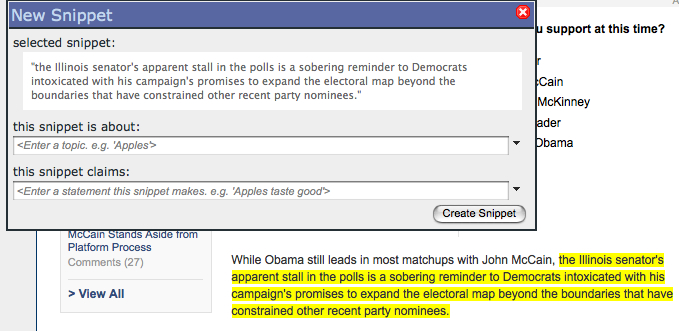
\includegraphics[scale=0.35]{../screenshots/snippetdialog_sm.jpg}
	\caption{Snippet creation dialog}
	\label{snippetdialog}
\end{figure}

\begin{figure}[ht]
	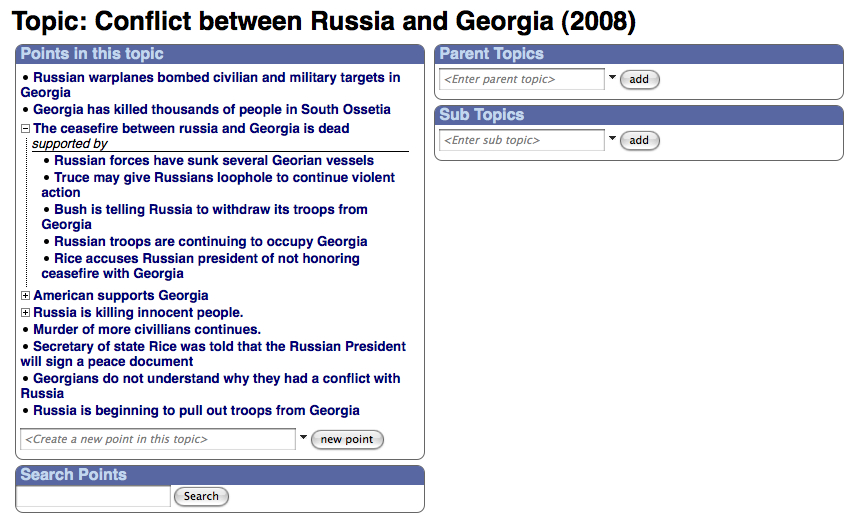
\includegraphics[scale=0.3]{../screenshots/topicpage_sm.jpg}
	\caption{Example topic page}
	\label{topicpage}
\end{figure}

\subsection{Implementation Decisions}

\idea{Wiki model not appropriate for points since want to manipulate several points at once}
\idea{Need to visualize relationships in web of ideas}


% \section{Creating Knowledge}
% 
% \section{Sharing Knowledge}
% 
% Why do users g
% 
% \section{Using Knowledge}
% 
% \section{Querying Data}


\section{User Studies}
1.5pp: recruitment, environment, tasks, observations, smaller study

\subsection{Recruitment}
Our user study participants were selected from a pool of respondents to a Craigslist posting for people who use the internet as one of their primary sources of information, regularly gather and share this information, and are interested in a new application to facilitate that process. We chose participants based on their responses to the following questions:
\begin{enumerate}
	\item What topics or types of information do you usually look for on the internet?
	\item How do usually go about finding information? (e.g. google, digg, friends, etc)
	\item How do you organize the information you find? (e.g. text file, paper, wiki, etc)
	\item How do you share information with others? (e.g. blog posts, comments, email, facebook, etc)
\end{enumerate}
We preferred individuals who search the internet for research and reading news rather than online shopping, as well as those interested in social and collaborative web activities like social networking web sites.  We were also interested in those who seemed to express a need for our application: people who copy-and-paste text from web pages into word processing documents, or who regularly email web page addresses to friends. Twelve people were selected to participate in this study.

\subsection{Study Environment}
Each study session lasted between thirty to forty-five minutes, with the participant sitting at a desktop computer with the Firefox browser running the application plugin. The session was a Think-Aloud study in which the participant verbally describes his/her thoughts throughout the duration of the study. A video camera captured the audio/video and was focused on the monitor screen. Before the session began, we briefly demonstrated the features of the application: how to (1) select snippets, (2) write a snippet topic and point, (3) relate points, (4) show/hide the margin, and (5) browse recent activity.

\subsection{Study Tasks}
The study consisted of two tasks to collect snippets, each lasting ten to fifteen minutes. During both tasks, we asked participants to browse the web as they normally would. In the first task, the participant browses the web about a topic or issue of their choice from the domain of politics. The collection of snippets should help the participant either argue or form an opinion/perspective about the topic, and should be thought of being used to help him/her explain or discuss the topic with a friend.  We constrained the first task to politics to increase the likelihood that the study participants would encounter similar issues and news stories.

For the second task, the participant was allowed to browse for any topic of their choosing. While the likelihood of topic overlap across participants was much lower, we were able to observe their behavior when searching for information in which each person had genuine interest.

At the conclusion of the session, we asked the participant if the application is something that would be likely to use, and for what purposes they would find it most useful. Any confusing features or experiences were also noted.

\subsection{Observations and Discussion}
% observed good and bad things
% good things validate the application's usefulness and applicability
% snippet selection super easy
% organization part a little lacking
% bad things we have ideas how to fix: UI redesign and smaller second study
% not as much social stuff going on, but limited stuff in DB for overlap to happen (more social stuff towards end of study)


{\it Note:} The first four study participants used a version of the web interface in which point relationships were constructed by navigating to one point page, searching for or typing the text of another point, and then expressing a directional relationship via a drop-down menu. We saw that participants found this process cumbersome and were less inclined to do it. Three of the four noted their confusion by the directional terms {\it supports} versus {\it is supported by}, and expressed a need for a more visual technique for constructing relationships. We modified the interface to allow users to drag and drop points on top of one another, with just the choice of {\it supports} and {\it opposes}. Half of the four participants were also confused by the Gmail-like labels alongside listed points that specified the topics each point belongs to.  The interface was modified to show topics listed with their related points beneath them. The remainder of the study used the modified interface. 

%hopefully more social uses when have more stuff in database

\subsubsection{Validating Observations?}
In general, the user study demonstrated that our application successfully allows people to associate portions of web content with ideas, and to organize and share those ideas. All the study participants were able to create new snippets, and only a couple ($2/12$) had initial difficulty in correctly summarizing snippet text into a point. Most participants ($10/12$) were interested in viewing the margin as they were creating new snippets. These observations demonstrate that snippet creation is easy for most users.

Many ($7/12$) participants also expressed the desire to organize snippets and points during their session. Of these seven, we noticed that four were alternating between creating snippets from new articles and organizing points in their {\it Recent Activity}: with each new snippet, users were creating relationships between points. When browsing web content about a particular topic or issue, most participants ($10/12$) either reused a topic that they created during their session or that someone else had created previously. Half of those ten used a topic that they {\it hadn't} created, demonstrating the ease of collaboration in our application. Both these organizational activities support connections inside the web of ideas. While the level of social activity was undoubtedly limited by the relatively small number of points (about $400$), three of the six people who browsed points in the main web interface looked at points created by other users. Two of the later study participants viewed someone else's point and either read the snippet text or viewed the originating document. As the number of points and topics increases, we expect to see more social behavior like this.

% easy to create snippets and view margin
% participants expressed desire to organize
% saw social activity and browsing
% (see more in usage types)
% not as much social stuff going on, but limited stuff in DB for overlap to happen (more social stuff towards end of study)

\subsubsection{Suggested Usage}
Many of the study participants who said they would our application suggested uses that match those described in our motivation, validating our prescribed use cases.  We identified the following use types, based on participant responses. Note that these many people suggested multiple use types.

\textbf{Blogging and writing:} Snippet collections are useful when gathering evidence and supporting material for a blog entry, report, or any kind of written composition. This use case necessitates the ability to organize, order, and rearrange snippets to best tell a story, generate a persuasive argument, or facilitate forming an opinion.

\textbf{Self-Bookmarking:} Creating snippets can be a means of bookmarking web page content that a user will return to for his/her own needs. These bookmarks are more specific than the web address of the page itself, and was suggested by users who currently find themselves cutting and pasting web content into a word processing file. This use case is more for retaining factual information than constructing an argument, although the information could also be used for the writing usage type.

\textbf{Social:} Sharing snippets with friends or targeted interest groups allows users to see what web content is interesting to people they follow. This use case is applicable both to those who wish to collaboratively generate a collection of information and to those who like sharing and browsing information from friends.

% Not for everyone! 3/12 people used it "incorrectly"
Several of the study participants suggested specific use cases that mirror our initial motivation for the application. One example was a user who would use snippets to as supporting evidence for asserting the incorrectness of someone else's claim on a web forum, as simple comments are not as effective. Our application, however, is not for everyone. Three of the twelve user study participants used (or wanted to use) our application ``incorrectly,'' e.g. to compare airline flight prices.

\subsubsection{User Interface Redesign}
The first user study demonstrated a few flaws in the application's user interface. These problems can be generalized as:
\begin{itemize}
	\item \textbf{People need to easily visualize the the hierarchy of points, topics, and relationships.} A significant portion of the participants ($5/12$) explicitly expressed confusion about not being able to view the entire hierarchy of topics and points, and felt lost when looking at the individual point or topic pages. In this view, each point and topic is visually separated from its related points and topics, and thus users did not understand the significance of these individual pages. Viewing related points as lists of {\it child} and {\it parent} points was confusing to three of the eight people who used the second version of the UI. This ``flattened'' perspective also makes it difficult to relate several points to another. Most of the users who linked points together ($5/7$) did not recognize the need to first create an intermediate point and then relate other points to that new point. An easier model for grouping and associating objects together is necessary.
	\item \textbf{People need better organization capabilities at snippet creation time.}
\end{itemize}

% motivation for file save-as in snippet dialog
\idea{people want to do most of their organization during the snippet creation process}
\idea{people want to be able to create subtopics right away}
\idea{specific topics used by different users are more likely not to be recreated}

Our solution to these problems was to redesign the user interface to resemble the traditional file browser. The left-hand side shows the expandable/collapsable hierarchy and shortcut paths, while the right-hand side shows a content preview of the selected item from the left. For example, when a point is selected, the preview shows its snippets and related points. Snippet creation will resemble a \texttt{save as...} dialog where users can easily traverse the topic/point hierarchy, and create new topics inside existing ones as deemed necessary.
This solution was implemented and used in a smaller user study. See section \ref{secondstudy}.


\subsubsection{Second User Study}
\label{secondstudy}
There were six study participants who used the redesigned web interface.
\studyresult{we solved organization difficulties with this redesign}

\section{Related Work}
1p

\subsection{Web Annotation Systems}

\subsection{Semantic Linking}

\subsection{User Contributed Links}

Memex allowed users to describe their own paths between pages, rather than requiring the page authors to modify them.

Everything2 creates soft-links between documents based on the browsing patterns of users.

ENQUIRE contains bi-directional links that show who links to a document. TrackBack does the same.

\subsection{Automated Reasoning}

\subsection{Argumentation Graphs}

%\section{Evaluation}

\section{Future Work}
1p: social queries, NLP stuff

\section{Conclusions}
$1/2$p

\end{document}